%%%%%%%%%%%%%%%%%%%%%%%%%%%%%%%%%%%%%%%%%
% Journal Article
% LaTeX Template
% Version 1.4 (15/5/16)
%
% This template has been downloaded from:
% http://www.LaTeXTemplates.com
%
% Original author:
% Frits Wenneker (http://www.howtotex.com) with extensive modifications by
% Vel (vel@LaTeXTemplates.com)
%
% License:
% CC BY-NC-SA 3.0 (http://creativecommons.org/licenses/by-nc-sa/3.0/)
%
%%%%%%%%%%%%%%%%%%%%%%%%%%%%%%%%%%%%%%%%%

%----------------------------------------------------------------------------------------
%	PACKAGES AND OTHER DOCUMENT CONFIGURATIONS
%----------------------------------------------------------------------------------------

\documentclass[twoside,twocolumn]{article}

\usepackage{blindtext} % Package to generate dummy text throughout this template 

\usepackage[sc]{mathpazo} % Use the Palatino font
\usepackage[T1]{fontenc} % Use 8-bit encoding that has 256 glyphs
\linespread{1.05} % Line spacing - Palatino needs more space between lines
\usepackage{microtype} % Slightly tweak font spacing for aesthetics

\usepackage[spanish]{babel} % Language hyphenation and typographical rules

\usepackage[hmarginratio=1:1,top=32mm,columnsep=20pt]{geometry} % Document margins
\usepackage[hang, small,labelfont=bf,up,textfont=it,up]{caption} % Custom captions under/above floats in tables or figures
\usepackage{booktabs} % Horizontal rules in tables

\usepackage{lettrine} % The lettrine is the first enlarged letter at the beginning of the text

\usepackage{enumitem} % Customized lists
\setlist[itemize]{noitemsep} % Make itemize lists more compact

\usepackage{abstract} % Allows abstract customization
\renewcommand{\abstractnamefont}{\normalfont\bfseries} % Set the "Abstract" text to bold
\renewcommand{\abstracttextfont}{\normalfont\small\itshape} % Set the abstract itself to small italic text

\usepackage{titlesec} % Allows customization of titles
\renewcommand\thesection{\Roman{section}} % Roman numerals for the sections
\renewcommand\thesubsection{\roman{subsection}} % roman numerals for subsections
\titleformat{\section}[block]{\large\scshape\centering}{\thesection.}{1em}{} % Change the look of the section titles
\titleformat{\subsection}[block]{\large}{\thesubsection.}{1em}{} % Change the look of the section titles

\usepackage{fancyhdr} % Headers and footers
\pagestyle{fancy} % All pages have headers and footers
\fancyhead{} % Blank out the default header
\fancyfoot{} % Blank out the default footer
\fancyhead[C]{Presentación de proyecto de ingeniería $\bullet$ Julio 2019 $\bullet$ Versión 2} % Custom header text
\fancyfoot[RO,LE]{\thepage} % Custom footer text

\usepackage{titling} % Customizing the title section

\usepackage{hyperref} % For hyperlinks in the PDF
\usepackage{apacite}
\bibliographystyle{apacite}
\usepackage{graphicx}
\usepackage{float}
\usepackage{siunitx}
\usepackage{amsmath}
%----------------------------------------------------------------------------------------
%	TITLE SECTION
%----------------------------------------------------------------------------------------

\setlength{\droptitle}{-4\baselineskip} % Move the title up

\pretitle{\begin{center}\Huge\bfseries} % Article title formatting
\posttitle{\end{center}} % Article title closing formatting
\title{Anteproyecto} % Article title
\author{%
\textsc{Diego José Orellana Bojorquez} \\[1ex] % Your name
\normalsize Universidad Rafael Landivar \\ % Your institution
\normalsize \href{mailto:djorellanab@outlook.com}{djorellanab@outlook.com} % Your email address
%\and % Uncomment if 2 authors are required, duplicate these 4 lines if more
%\textsc{Jane Smith}\thanks{Corresponding author} \\[1ex] % Second author's name
%\normalsize University of Utah \\ % Second author's institution
%\normalsize \href{mailto:jane@smith.com}{jane@smith.com} % Second author's email address
}
\date{\today} % Leave empty to omit a date
\renewcommand{\maketitlehookd}{%
\begin{abstract}
En la presente publicación se presenta los detalles para realizar el proyecto de graduación, \textbf{Análisis de la Interfaz de Programación de Aplicaciones (API) del dispositivo Kinect V2 para la detección de los pasos de un movimiento.}
\medbreak
\textbf{Descriptores:} Kinect V2, Sedentarismo, Reconocimiento de movimiento Y Seguimiento de esqueleto
\end{abstract}
}

%----------------------------------------------------------------------------------------
\begin{document}

% Print the title
\maketitle

%----------------------------------------------------------------------------------------
%	Contenido del artículo
%----------------------------------------------------------------------------------------

\section{Introducción}

El sedentarismo es un modo de vida orientado al poco ejercicio que realizan una persona, además de ser una de las causas de enfermedades no transmisibles, como la diabetes. Por lo tanto, en la presente publicación se presenta el detalle del proyecto final de Ingeniería en informática y sistemas, la cual consta de realizar un prototipo que reconozca un movimiento, además de realizar una evaluación de la actividad de física de una persona a partir del conteo de repeticiones del movimiento.

%------------------------------------------------
\section{Justificación}
El sedentarismo es una de las principales causas de la obesidad y sobrepeso en Guatemala, as\'i mismo constituye un factor determinante para el desarrollo de enfermedades cr\'onicas no transmisibles, concretamente la diabetes, tal como se muestra en el estudio m\'edico, Risk to Develop Type 2 Diabetes Mellitus according to FINDRISC tool in Guatemalan Physicians aged 40-60 years \cite{castro2017risk}, menciona que el 47\% de los guatemaltecos con diabetes tiene problemas de obesidad y el 31\%  sufren de problemas de sobrepeso, por lo cual refleja la inactividad f\'isica en una gran parte de la poblaci\'on guatemalteca.
\medbreak
Por otra parte, se ha reducido el nivel de actividad f\'isica en las personas guatemaltecas, tal como se menciona en la encuesta de diabetes, hipertensi\'on y factores de riesgo de enfermedades cr\'onicas \cite{orellana2006organizacion}, el 27.68\% de los guatemaltecos presenta sedentarismo, debido que no realiza actividades f\'isicas o lo hacen por menos de 30 minutos.
\medbreak
Igualmente, se realiz\'o un estudio a 392 ni\~nos y adolescentes en escuelas rulares y urbanas de Guatemala \cite{orellana2006organizacion}, en donde indica que alrededor del 62\% de los ni\~nos del  \'area urbana presenta problemas de sobrepeso y un 13.8\% de obesidad, de modo que los autores concluyeron que el sobrepeso y la obesidad coexisten en los ni\~nos y adolescentes guatemaltecos.
\medbreak
En resumen, el presente proyecto brindar\'a una soluci\'on innovadora y tecnol\'ogica para evaluar la actividad f\'isica en los guatemaltecos, a partir de la detecci\'on de los pasos para realizar una movimiento. De tal modo de responder la siguiente pregunta:
\medbreak
\begin{center}
\textbf{?`Será posible contabilizar el sedentarismo de una persona, a partir de la actividad física de un movimiento?}
\end{center}
\section{Estudios relacionados}
\subsection{Sistema de detecci\'on y reconocimiento de la postura corporal basado en Kinect}
\citeA{pisharady2013kinect} mencionan que alrededor del 66\% de la poblaci\'on mundial  utilizan la comunicaci\'on no verbal, dicha comunicaci\'on esta conformado por posturas corporales, gestos, expresiones faciales y movimientos corporales. Por lo tanto, los autores propone un sistema para detectar expresiones est\'aticas -i.e. Posiciones que no cambian durante un per\'iodo de expresi\'on-.
\medbreak
Dicho sistema detecta y reconoce posturas corporales de una persona con la ayuda del sensor del Kinect, ya que le proporciona la posici\'on de las articulaciones del cuerpo humano -e.g. mano, codo, hombro, rodilla- en un espacio vectorial definido por el sensor. Posteriormente se calcula las caracter\'isticas angulares respecto a dos vectores de articulaciones, por ejemplo; para encontrar la caracter\'istica angular del codo derecho se utiliza los vectores de la mano derecha y hombro derecho.
\medbreak
Por otro lado, \citeA{pisharady2013kinect} analizaron un total de 11 componentes angulares para entrenar una m\'aquina de soporte vectorial -i.e SVM- de n\'ucleo polin\'omico, con la finalidad de detectar un total de 10 movimientos est\'aticos -e.g. Pararse, agacharse, hablar por tel\'efono-, as\'i mismo el entrenamiento consisti\'o en tomar 6000 muestras de posturas de 6 personas diferentes -i.e. Cada persona realiz\'o 100 muestras por postura-.
\medbreak
Finalmente, \citeA{pisharady2013kinect} recolectaron un total de 5000 muestras positivas -i.e. Correspondiente a los 10 movimientos est\'aticos-. Como resultados obtuvieron una falla de pron\'ostico de 1.46\%, debido que el sensor Kinect no podr\'ia rastrear correctamente el seguimiento esqueleto.
\subsection{Reconstruci\'on de posturas en tiempo real} \label{tr:2}
\citeA{shum2013real} determinaron que el sensor Kinect tiene un problema con el reconocimiento de postura a la hora de interactuar con objetos externos -e.g. Baloncesto, levantamiento pesas-, por lo tanto, algunos datos de seguimiento de esqueleto son incorrecto, de tal manera que lo autores propone un m\'etodo para medir la confiabilidad de datos al momento de detectar una postura.
\medbreak
Para determinar el nivel de confiabilidad de datos, \citeA{shum2013real}, contruyeron una base de datos de 21590 posturas est\'aticas, la cual mide los \'angulos entre articulaciones. Esto permite  extraer las 30 posturas que se asemeja al movimiento real -i.e. 30 vecinos m\'as cercanos-.  Posteriormente, localizan cada postura en un nuevo espacio vectorial -i.e Espacio diferente al Kinect-, seleccionando as\'i la postura que tenga uno menor distancia entre los puntos vectoriales.
\medbreak
Finalmente, \citeA{shum2013real}, realizaron las pruebas a 27 personas, dichas pruebas consist\'ia en hacer actividades con objetos externos -e.g. caja, silla, l\'apiz, pelota-, analizando la parte superior -i.e. Arriba de la caderas- e inferior de cada persona. Como resultados a estas pruebas, encontraron una diferencia de distancia -i.e. Entre la postura real y de referencia- de 9 a 13 cm, determinando as\'i un nivel de confiabilidad del de 80\% respecto a dos sistemas de detecci\'on de movimiento en tiempo real \cite{shum2011fast,shum2012real}.
\subsection{Detecci\'on de posturas a la hora de sentarse para prevenir el s\'indrome de los trabajadores de oficina usando el Kinect} \label{tr:3}
\citeA{paliyawan2014prolonged} estudiaron el s\'indrome del trabajador de oficina, la cual consiste en un grupo de s\'intomas que tiene los trabajadores por los h\'abitos no saludables -e.g. La postura a la hora de sentarse-, provocando en la persona distintos dolores corporales -e.g. Muscular, sequedad en los ojos-.
\medbreak
En relaci\'on a los riesgos de salud de una persona, \citeA{paliyawan2014prolonged}, investigaron que una de las causas de las enfermedades no transmisible es debido al tiempo prolongado de estar sentado, sin realizar ning\'una actividad f\'isica. Por lo tanto, los autores  proponen un sistema que detecta las posturas a la hora que esta trabajando en una oficina.
\medbreak
Para realizar dicho sistema, \citeA{paliyawan2014prolonged} estudiaron las posturas de 28 personas,  recolectaron un total de 1326 posturas. De igual manera, cada postura conten\'ia un total 31 atributos -i.e. Tiempo y posici\'on de 10 articulaciones-. Posteriormente, el sistema procesa los datos y encuentra la distancia euclidiana entre los datos consecutivos, permitiendo normalizar las distancias m\'aximas y m\'inimas por persona y en forma general -i.e. Conjunto de personas analizadas-.
\medbreak
Finalmente, el sistema detecta una buena o mala posici\'on, a partir de cuatros m\'etodos de clasificaci\'on: \'Arboles de decisiones, redes neuronales, clasificador bayesiano y 5 vecinos m\'as cercanos. Por lo tanto, para seleccionar el mejor m\'etodo, los autores realizaron una prueba a 10 personas, de tal manera que el mejor  clasificador es de los vecinos m\'as cercano, debido que tuvo una precisi\'on de  98.83\%. 
\subsection{Una comparaci\'on entre las t\'ecnicas heur\'isticas y de aprendizaje autom\'atico en la detecci\'on de ca\'idas con Kinect v2} \label{tr:7}
En la publicaci\'on, A Comparison Between Heuristic And Machine Learning Techniques In Fall Detection Using Kinect v2 \cite{amini2016comparison}, se compara 2 m\'etodos para detectar la posici\'on, velocidad y aceleraci\'on de un usuario al momento de que un usuario sufre de una ca\'ida.
\medbreak 
Seg\'un \citeA{amini2016comparison}, el primer m\'etodo se basa en la heur\'istica que aprovecha la funcionalidad del seguimiento de esqueleto, la cual consiste en analizar la distancia entre la articulaci\'on de la cabeza y el suelo -i.e. Recta respecto a las articulaciones de los p\'ies-, mientras que el segundo m\'etodo consiste en una m\'aquina de aprendizaje, usando la funcionalidad visual y constructor de gestos -i.e. VGB-, la cual analiza el escenario y le asigna un color -i.e. en escala RGB- a las posibles fallas de ca\'idas.
\medbreak 
As\'i mismo, \citeA{amini2016comparison} mencionan que para el primer m\'etodo los datos se fueron determinando a partir de la ecuaci\'on escalar de un plano, mientras que en el segundo m\'etodo se utiliz\'o el algoritmo AdaBoostTrigger -i.e Modelo discreto de VGB-.
\medbreak 
Finalmente, \citeA{amini2016comparison} realizaron una prueba con 11 personas, la cual concluyeron que para el primer m\'etodo detectaba un 95.42\% de las ca\'idas, mientras que para el segundo m\'etodo fue de 88.33\%, por lo tanto el primer m\'etodo era m\'as exacto debido que no depend\'ia tanto de los datos de entrenamiento -i.e El usuario no replicaba los v\'ideos de entrenamiento del modelo VGB-.
\section{Objetivos}
\subsection{General}
Implementar un modelo de pronóstico de detección de los pasos que debe seguir para realizar un movimiento, con la ayuda de las herramientas proporcionada por la interfaz de programación de aplicaciones del dispositivo Kinect V2.
\subsection{Específicos}
\begin{itemize}
\item Definir el movimiento a analizar, considerando los pasos que se debe seguir para realizar dicho movimiento.
\item Desarrollar una rutina del movimiento, para la captura de datos.
\item Identificar la distancia mínima y máxima de profundidad entre el Kinect y el usuario para la detección del seguimiento de esqueleto.
\item Recolectar los datos de la rutina del movimiento, a partir de la herramienta Kinect Studio.
\item Crear una base de datos de reconocimiento de gesturas y posturas,  por medio de la herramienta Visual Gesture Builder y los datos recolectado del Kinect Studio.
\item Calcular los errores del pronostico del reconocimiento de gesturas y posturas.
\item Crear una interfaz gráfica que detecte las repeticiones realizada del movimiento.
\item Crear una interfaz gráfica que demuestre los resultados de un entrenamiento.
\item Comprobar el modelo de reconocimiento de gesturas y posturas del movimiento.
\end{itemize}
\section{Hipótesis}
Un software que mida el sedentarismo a partir de la actividad física de una persona.
\section{Metodología}
Para el presente proyecto se debe seleccionar un movimiento, describiendo todos los pasos respectivo del movimiento, además de las articulaciones que interviene para realizar el movimiento, por ejemplo: Air Squat:
\begin{table}[H]
\caption{Análisis del movimiento}
\centering
\begin{tabular}{llr}
\toprule
\multicolumn{2}{c}{Air Squat} \\
\cmidrule(r){1-2}
Joints & Rodilla derecha e izquierda \\
     & Tobillo derecho e izquierdo \\
     & cadera derecha e izquierda \\
     & Espalda \\
\cmidrule(r){1-2}
Paso & Descripción \\
\midrule
1 & Párese con los pies ligeramente      \\
  & más separados que el ancho de        \\
  & los hombros, manteniendo el          \\
  & peso  sobre los talones y los pies 	 \\
  & inclinados ligeramente hacia afuera. \\
2 & Coloque sus brazos frente a su pecho \\
  & en una posición cómoda. Empieza a    \\
  & doblar las rodillas para bajar       \\
  & hacia el suelo. Su espalda debe      \\
  & permanecer recta. 					 \\
3 & Continúa doblando las rodillas       \\
  & hasta que los muslos estén           \\
  & paralelos al suelo.                  \\
\bottomrule
\end{tabular}
\textbf{Fuente:} \citeA{withfitAirSquat}
\end{table}
\medbreak 
Posteriormente a la definición del movimiento, se debe crear una rutina del ejercicios tomando en cuenta los factores que puede llegar a intervenir -e.g. Estiramiento, Calentamiento, Práctica del movimiento-, permitiendo simular el ambiente de una rutina, tal como se muestra el siguiente ejemplo:
\begin{table}[H]
\caption{Ejemplo de Rutina de ejercicio}
\centering
\begin{tabular}{llr}
\toprule
\multicolumn{2}{c}{Rutina de Air Squat} \\
\midrule
Tiempo & 2 minutos                       \\
Trabajo & Realizar las máximas           \\
        & repeticiones posibles de Air   \\
        & Squat durante el tiempo        \\
        & asignado.                      \\
\bottomrule
\end{tabular}
\textbf{Fuente:} Autor del anteproyecto
\end{table}
\medbreak 
Una vez definido la rutina del movimiento, se debe encontrar la distancia de profundidad entre el usuario y el Kinect, en donde se genere correctamente el seguimiento de esqueleto del usuario al momento de realizar el movimiento, tal como se observa en la siguiente figura.
\begin{figure}[H]
	\caption{Visualización de captura de datos}
	\label{fig:capturaDatos}
	\centering
	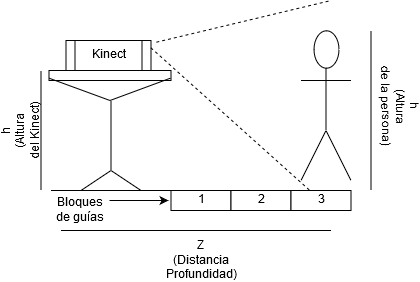
\includegraphics[width=170px,height=100px]{img/RecoleccionProfundidad.png} \\
	\textbf{Fuente:} Elaboración propia
\end{figure}
En la figura \ref{fig:capturaDatos}, se observa las siguientes variables:
\begin{itemize}
\item \textbf{La altura del kinect respecto el suelo}: esta variable permanecerá constante por movimiento.
\item \textbf{La altura del usuario}: Se calculará respecto la posición de altura de las articulaciones: Cabeza y pies del usuario.
\item \textbf{Distancia entre el usuario y Kinect}: Distancia de profundidad respecto el Kinect y el punto de articulación de análisis -e.g. Centro de cadera, Centro de hombro, Espalda-.
\item \textbf{Bloques guías}: Enumeración de rangos de profundidad para realizar el movimiento.
\begin{table}[H]
\caption{Ejemplo de bloques guías}
\centering
\begin{tabular}{lllr}
\toprule
bloque & inferior & superior  \\
\midrule
1 & 0 cm  & 60 cm             \\
2 & 60 cm & 120 cm            \\
3 & 120 cm & 180 cm           \\
4 & 180 cm & 240 cm           \\
5 & 240 cm & 300 cm           \\
6 & 300 cm & 360 cm           \\
\bottomrule
\end{tabular}
\end{table}
\end{itemize}
\medbreak 
Una vez finalizado la toma de datos de distancia de profundidad, se realizará una tabla de frecuencia, para determinar la distancia mínima y máxima para realizar el movimiento correspondiente:
\begin{table}[H]
\caption{Ejemplo de tablas de frecuencias}
\centering
\begin{tabular}{lllr}
\toprule
Articulación & \multicolumn{2}{c}{Centro de los hombros} \\
\midrule
bloque & altura & frecuencia \\
1 & 0 cm & 0             \\
2 & 0 cm & 0             \\
3 & 0 cm & 0		     \\ 
4 & 0 cm & 0       \\
5 & 120 cm a 160 cm & 20 \\
6 & 160 cm a 200 cm & 10 \\
\bottomrule
\end{tabular}
\end{table}
\medbreak 
Tal como se observa en el ejemplo de tabla de frecuencia, se puede determinar que el seguimiento de esqueleto del movimiento se genera correctamente a una distancia mínima de 240 cm hasta una distancia máxima de 360 cm -i.e. Entre los bloques guías 5 y 6-.
\medbreak 
Luego de encontrar las distancia de profundidad, se posicionará la persona y se grabará un vídeo realizando la rutina del movimiento, a partir de la herramienta Microsoft Kinect Studio:
\begin{figure}[H]
	\caption{Ejemplo de vídeo del Kinect Studio}
	\label{fig:KinectStudio}
	\centering
	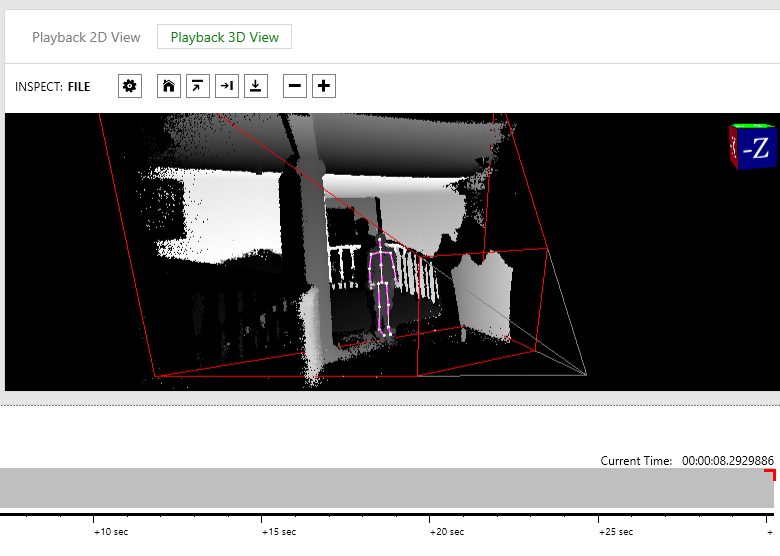
\includegraphics[width=170px,height=100px]{img/kinectStudio.PNG} \\
	\textbf{Fuente:} Tomado por el autor
\end{figure}
\medbreak 
Terminando la recolección de datos de vídeo, se le asignará una etiqueta a cada paso correspondiente del movimiento, dicha etiqueta tendrá un valor entre 0 a 1 -i.e. Valor pronóstico-, tal como se observa en la siguiente tabla:
\begin{table}[H]
\caption{Etiquetas de ejemplo}
\centering
\begin{tabular}{llr}
\toprule
\multicolumn{2}{c}{Air Squat} \\
\midrule
Pasos & 3  \\
\midrule
Offset & 1/(3-1) = 0.5   \\
\midrule
Paso & Etiqueta \\
\midrule
1 & 0.0    \\
2 & 0.5    \\
3 & 1.0    \\
\bottomrule
\end{tabular}
\end{table}
\textbf{Fuente:} Autor del anteproyecto
\medbreak 
Esta tabla es un ejemplo que permite asignarle etiquetas al modelo de pronóstico para la detección del paso del movimiento -e.g. Cuando el valor es cercano a 0, se reconoce el paso 1-, tomando en cuenta las variables de: distancias, velocidades y  aceleraciones de cada articulación capturado en el seguimiento de esqueleto.
\medbreak 
Para realizar el modelo de pronóstico de detección de paso del movimiento, se creará una base de datos de reconocimientos de gesturas y posturas, con la herramienta Visual Gesture Builder, la cual se analizará los vídeos generado por el Kinect Studio, y se le asignará el valor de la etiqueta del paso, en el momento del vídeo que se esta realizando, tal como se muestra en las siguientes figuras:
\begin{figure}[H]
	\caption{Asignación paso 1}
	\label{fig:Paso1}
	\centering
	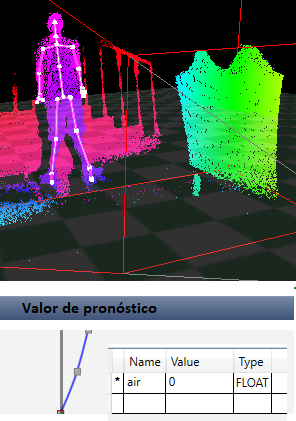
\includegraphics[width=170px,height=120px]{img/paso1.PNG} \\
	\textbf{Fuente:} Tomado por el autor
\end{figure}
\begin{figure}[H]
	\caption{Asignación paso 2}
	\label{fig:Paso2}
	\centering
	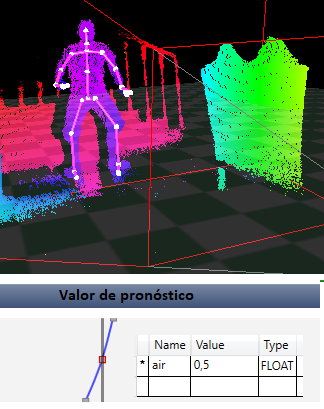
\includegraphics[width=170px,height=120px]{img/paso2.PNG} \\
	\textbf{Fuente:} Tomado por el autor
\end{figure}
\medbreak 
\begin{figure}[H]
	\caption{Asignación paso 3}
	\label{fig:Paso3}
	\centering
	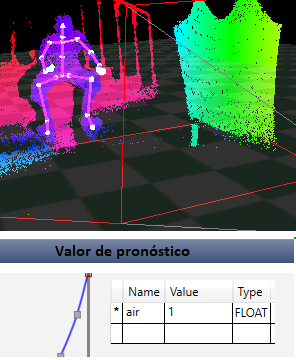
\includegraphics[width=170px,height=120px]{img/paso3.PNG} \\
	\textbf{Fuente:} Tomado por el autor
\end{figure}
\medbreak
Concluyendo con la asignación de etiquetas de cada vídeo, se utilizará cierta cantidad de datos para el entrenamiento y compilación de la base de datos de gesturas y posiciones del movimiento. Y así mismo los datos que sobran -i.e. Datos de pruebas- será utilizado por la herramienta de análisis de Visual Gesture Builder, que proporcionará el valor de pronóstico y el valor esperado:
\begin{figure}[H]
	\caption{Resultado de Gesturas}
	\label{fig:resultados}
	\centering
	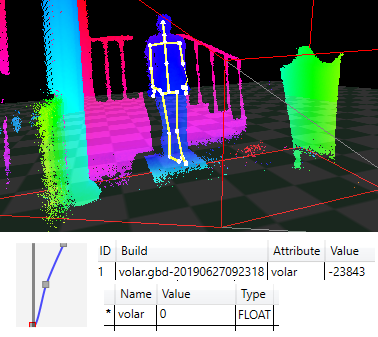
\includegraphics[width=170px,height=120px]{img/resultado.PNG} \\
	\textbf{Fuente:} Tomado por el autor
\end{figure}
\medbreak
En la figura de resultados de gesturas, se observa que el valor esperado es de 0.000000, mientras que el valor de pronóstico es de \num{-23843e-6}, por lo tanto se va a tabular los valores esperados y pronosticado por cada frame de cada vídeo de prueba, y a partir de estos valores se determinará los siguientes errores del pronóstico:
\[
 \begin{matrix}
  Y_t & Esperado \\
  Y'_t & Pronosticado \\
  e_t & Y_t - Y_t' \\
  t & id \\
  n & TotalDeDatos
 \end{matrix}
\]
\begin{itemize}
\item \textbf{Error medio del pronóstico (EMP)}
\[
	EMP = \frac{\sum_{t=1}^{n} e_t}{n}
\]
\item \textbf{Error medio al cuadrado (EMC)}
\[
	EMC = \frac{\sum_{t=1}^{n} (e_t)^2}{n}
\]
\item \textbf{Desviación estándar de los errores (DDE)} 
\[
	DDE = \sqrt{\frac{\sum_{t=1}^{n} (e_t-EMP)^2}{n-1}}
\]
\item \textbf{Desviación absoluta de la media (DAM)} 
\[
	DAM = \frac{\sum_{t=1}^{n} |e_t|}{n}
\]
\item \textbf{Porcentaje de error medio absoluto (PEMA)}
\[
	PEMA = \frac{\sum_{t=1}^{n} |\frac{e_t}{Y_t}|*100}{n}
\]
\end{itemize}
De igual manera, es necesario probar distintos modelos de pronóstico de gesturas y posiciones de un movimiento para identificar el modelo que tenga un menor error, por lo tanto se utilizará la técnica de cross validation:
\begin{table}[H]
\caption{Ejemplo de cross validation}
\centering
\begin{tabular}{llllr}
\toprule
Folds & 1 & 2 & 3 & 4 \\
Datos & 25\% & 25\% & 25\% & 25\% \\
\midrule
\#  &  \multicolumn{2}{c}{Folds build} & \multicolumn{2}{c}{Fold Test} \\
1  & \multicolumn{2}{c}{1 2 3} & \multicolumn{2}{c}{4}\\
2  & \multicolumn{2}{c}{1 2 4} & \multicolumn{2}{c}{3}\\
3  & \multicolumn{2}{c}{1 3 4} & \multicolumn{2}{c}{2}\\
4  & \multicolumn{2}{c}{2 3 4} & \multicolumn{2}{c}{1}\\
\bottomrule
\end{tabular}
\end{table}
\medbreak 
En la tabla de ejemplo de cross validation, se separa en 4 Folds, la cual cada Fold contiene el 25\% de los datos capturados, de igual manera se divide en 4 modelos de pronóstico de gesturas y posiciones, por cada modelo se utilizará el 75\% de los datos para construirlo y el 25\% de pruebas, así mismo se debe calcular los respectivos errores de pronóstico:
\begin{table}[H]
\caption{Ejemplo de errores calculado en cross validation}
\centering
\begin{tabular}{lllllr}
\toprule
\# & EMP & EMC & DEE & DAM & PEMA \\
\midrule
1 & 2.60  & 230 & 11.7 & 8.40 & 12.0\% \\
2 & 1.00  & 180 & 8.4  & 7.30 & 9.4\%  \\
3 & -4.10 & 240 & 10.5 & 7.90 & 11.0\% \\
4 & -2.00 & 260 & 12.3 & 9.97 & 13.4\% \\
\bottomrule
\end{tabular}
\end{table}
\medbreak 
Para el presente ejemplo se seleccionará el modelo 2, debido que contiene un menor error comparado con los demás modelos, así mismo se puede determinar la información necesaria para reconocer el movimiento:
\[
 \begin{matrix}
  E & Etiqueta \\
  off & Offset \\
  err & Error
 \end{matrix}
\]
\[ min(E) =
  \begin{cases}
    E               & \quad \text{Primera E}\\
    E-(of*er/2)     & \quad \text{E's del medio}\\
    E-(of*er)       & \quad \text{Ultima E}\\
  \end{cases}
\]
\[ max(E) =
  \begin{cases}
    E+(of*er)       & \quad \text{Primera E}\\
    E+(of*er/2)     & \quad \text{E's del medio}\\
    E               & \quad \text{Ultima E}\\
  \end{cases}
\]
\begin{table}[H]
\caption{Ejemplo de metadata del movimiento}
\centering
\begin{tabular}{lllr}
\toprule
\multicolumn{2}{c}{Nombre}  & \multicolumn{2}{c}{Air Squat}\\
\midrule
\multicolumn{2}{c}{Pasos}   & \multicolumn{2}{c}{3} 		   \\
\midrule
\multicolumn{2}{c}{Joints}   & \multicolumn{2}{c}{Tobillo derecho,} 		   \\
\multicolumn{2}{c}{}   & \multicolumn{2}{c}{Tobillo izquierdo} 		   \\
\multicolumn{2}{c}{}   & \multicolumn{2}{c}{Rodilla derecha} 		   \\
\multicolumn{2}{c}{}   & \multicolumn{2}{c}{Rodilla izquierda} 		   \\
\multicolumn{2}{c}{}   & \multicolumn{2}{c}{Cadera derecha} 		   \\
\multicolumn{2}{c}{}   & \multicolumn{2}{c}{Cadera  izquierda} 		   \\
\multicolumn{2}{c}{}   & \multicolumn{2}{c}{Espalda} 		   \\
\midrule
\multicolumn{2}{c}{Articulación}   & \multicolumn{2}{c}{Centro} 		   \\
\multicolumn{2}{c}{de}   & \multicolumn{2}{c}{de los} 		   \\
\multicolumn{2}{c}{análisis}   & \multicolumn{2}{c}{hombros} 		   \\
\midrule
\multicolumn{2}{c}{Profundidad Mínima}   & \multicolumn{2}{c}{240 cm} 	 \\
\midrule
\multicolumn{2}{c}{Profundidad Máxima}   & \multicolumn{2}{c}{360 cm} 		   \\
\midrule
\multicolumn{2}{c}{off}  & \multicolumn{2}{c}{0.5} 	   \\
\midrule
\multicolumn{2}{c}{Modelo}  & \multicolumn{2}{c}{2} 		   \\
\midrule
\multicolumn{2}{c}{err}   & \multicolumn{2}{c}{9.4\%}    \\
\midrule
Paso    & E        & Min    & Max        \\
1 		& 0   	   & 0 	    & 0.0470     \\
2 		& 0.5      & 0.4765 & 0.5235     \\
3 		& 1        & 0.9530 & 1.0000     \\
\bottomrule
\end{tabular}
\end{table}
\medbreak 
Tal como se observar en la tabla, si la probabilidad de pronóstico se encuentra en el intervalo de 0 a 0.0470, va reconocer el paso 1, de igual manera es necesario reconocer las repeticiones del movimiento por lo cual debe seguir el siguiente algoritmo:
\begin{figure}[H]
	\caption{Algoritmo reconocimiento de repeticion}
	\label{fig:algoritmo}
	\centering
	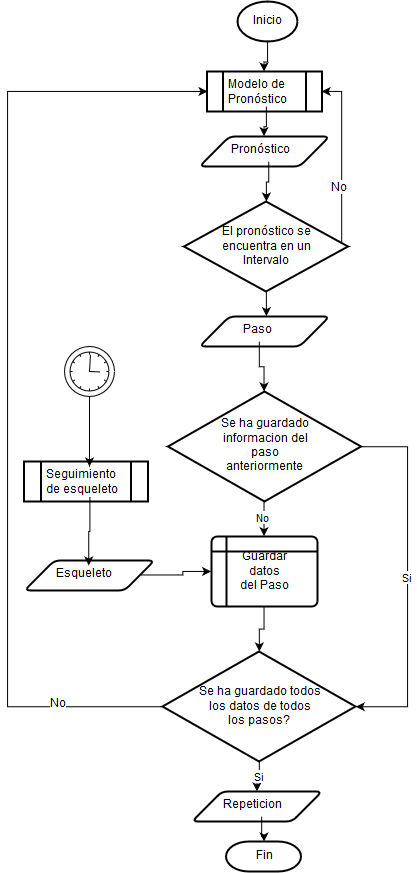
\includegraphics[width=170px,height=350px]{img/algoritmo.png} \\
	\textbf{Fuente:} realizado por el autor
\end{figure}
\medbreak 
Tal como se observar en el algoritmo, se va a reconocer una repetición, siempre cuando el usuario haya pasado por todos los pasos correspondiente del movimiento, Así mismo por cada paso se va almacenar datos del esqueleto:
\[
 \begin{matrix}
  ID & Repeticion:Entero                   \\
  SE & Serie:Entero                        \\
  S & Paso:Entero                          \\
  p & probabilidad:Decimal                 \\
  A & Articulacion:Entero                  \\
  T & Tiempo(Segs):Decimal                 \\
  x & Ancho(Pixeles):Decimal               \\
  y & Altura(Pixeles):Decimal
 \end{matrix}
\]
Una vez identificado las repeticiones y los datos que se va almacenar, será necesario realizar una interfaz gráfica, en donde permita detectar los pasos del movimiento y las repeticiones que realiza en un período de tiempo:
\begin{figure}[H]
	\caption{Interfaz gráfica de reconocimiento de movimiento}
	\label{fig:resultados}
	\centering
	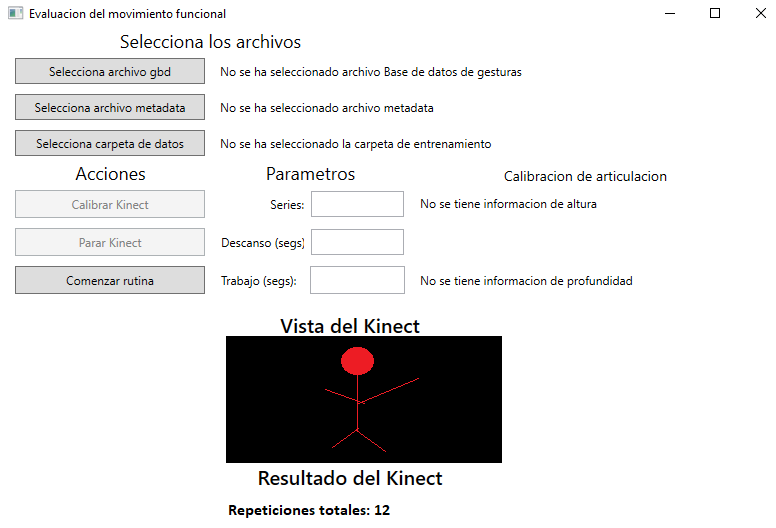
\includegraphics[width=170px,height=120px]{img/evaluation.PNG} \\
	\textbf{Fuente:} Tomado por el autor
\end{figure}
La interfaz gráfica será implementada en Windows Presentation Foundation -i.e. WPF-. En dicha interfaz se debe adjuntar la base de datos de Gesturas, realizada por el Visual Gesture Builder,  y la información extra del movimiento -i.e. Archivo de metadata en formato JSON-. Además de indicar  los parámetros de la rutina del ejercicio -i.e. Tabata-: Tiempo de trabajo, Tiempo de descanso y la cantidad de series.
\medbreak 
Teniendo todos estos parámetros de configuración, el usuario puede empezar la rutina en la distancia de profundidad recomendada -i.e. Para el presente ejemplo sería una distancia de 240 a 360 cm-, la cual se le mostrará en tiempo real la imagen del seguimiento de esqueleto  -i.e. Imagen en 2 Dimensiones-, Así mismo el usuario debe realizar las máximas repeticiones posibles durante el tiempo de trabajo. Una vez finalizado la rutina, se exportará un archivo con los siguientes resultados:
\begin{itemize}
\item Tiempo de descanso
\item Tiempo de trabajo
\item Cantidad de series
\item Volumen de repeticiones
\item Duración total de la rutina
\item Repeticiones máxima durante un período de tiempo mínimo
\item Repeticiones promedio por serie
\item Tiempo promedio por repetición
\item Tiempo promedio entre dos pasos seguidos.
\item Flexibilidad promedio de cada articulación por cada paso.
\item Distancia promedio de cada articulación entre dos pasos seguidos.
\end{itemize}
Finalmente se debe crear una interfaz gráfica que muestre todos los resultados respectivos de la rutina de una manera visual:
\begin{figure}[H]
	\caption{Ejemplo de tabata de Air Squat}
	\label{fig:hiit}
	\centering
	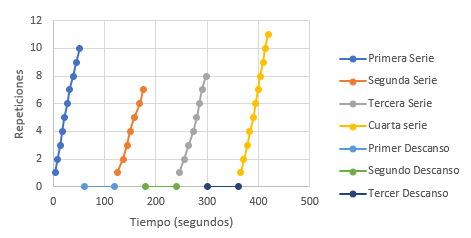
\includegraphics[width=170px,height=120px]{img/hiitMf.PNG} \\
	\textbf{Fuente:} Realizado por el autor
\end{figure}
\medbreak
En el ejemplo visual de Tabata, mide la actividad física de una persona, a partir de repeticiones del movimiento, Air Squat. Se debe tomar en cuenta que la rutina de ejemplo se configuró 4 series de 60 segundos de trabajo y 60 segundos de descanso, realizando un total de 36 repeticiones durante 480 segundos.
\medbreak
Finalmente para comprobar el modelo de reconocimiento de gesturas y posturas del movimiento, se realizará un conjunto de evaluaciones -i.e. Todas las evaluaciones tendrá configurada los mismos parámetros-. 
\medbreak
Así mismo en cada evaluación, habrá una persona contando las repeticiones respectivas por series y finalmente se va a comparar contra las repeticiones del software, tal como se observa en las siguiente tabla:
\begin{table}[H]
\caption{Ejemplo de validación de movimiento}
\centering
\begin{tabular}{llr}
\toprule
\multicolumn{2}{c}{Air Squat} \\
\midrule
Repeticiones & Repeticiones \\
esperada &  Pronosticada \\
\midrule
10 & 10    \\
9 & 8    \\
11 & 12    \\
\bottomrule
\end{tabular}
\end{table}
\textbf{Fuente:} Autor del anteproyecto
\medbreak 
El motivo de esta tabulación de datos, es para encontrar el error de detección de repetición del movimiento -i.e. Desviación estándar-.
%------------------------------------------------

%------------------------------------------------
\section{Recursos}
\subsection{Tecnológicos}
\begin{itemize}
\item Sensor Kinect XBox One -i.e. V2-.
\item Adaptador del sensor Kinect.
\item Kinect SDK V2
\item Computadora -i.e. Procesamiento, almacenamiento y memoria suficiente para ejecutar el Kinect SDK V2-.
\end{itemize}
\subsection{Educativos}
\begin{itemize}
\item IDE: Licenciamiento de Visual Studio professional
\item IDE: Visual Studio Code
\item Github Education
\item Licenciamiento de Visual Studio professional 
\end{itemize}
\subsection{Humanos}
\begin{itemize}
\item Departamento de deportes de la Universidad Rafael Landívar
\end{itemize}
\section{Validaciones}
\citeA{sedentarismoOMS}, define actividad sedentaria como una actividad que no realiza la actividad física, así mismo se considera actividad física a cualquier movimiento corporal producido por los músculos esqueléticos que exija gasto de energía \cite{actividadFisicaOMS}. De igual manera el gasto de energía se presenta al momento de que un músculo se contrae, ya que se liberan moléculas llamadas, Adenosín Trifosfato -i.e. ATP-, dicha molécula se puede metabolizar de tres formas distintas \cite[p.~195]{marieb2008anatomia}:
\begin{enumerate}
	\item \textbf{Fosforilación directa:} Al momento de realizar una actividad intensa -e.g. Corrida de 100 mts, durante un período de 15 segundos-.
	\item \textbf{Respiración aeróbica:} Al momento que los músculos se encuentra en reposo o realiza un ejercicio leve -i.e. Cuando una persona mira la televisión-.
	\item \textbf{Glucólisis anaeróbico y formación de ácido láctico:}  Al momento que los músculos realiza una actividad moderada -i.e. Cuando una persona realiza repeticiones de sentadillas durante un período de 1 a 2 minuto-.
\end{enumerate}
Tal como se observa, las moléculas de energía se  metabolizan al momento de realizar una actividad física, dicha actividad puede ser programados a partir de rutinas, como por ejemplo el Tabata -i.e. Rutina de ejercicio de alta intensidad-, la cual consta de un entrenamiento de series de tiempo de descanso y de trabajo, en donde la persona debe hacer las máxima cantidad de repeticiones posible de un movimiento durante el tiempo de trabajo. Por lo tanto esta rutina puede llegar a producir grandes cantidades de moléculas de energía, ya que en el año 1996, el japonés científico, Izumi Tabata, comparó una rutina intensa de 4 minutos contra una rutina tradicional de 60 minutos, por medio del volumen de oxigeno que puede procesar el cuerpo humano. En donde observó que para la rutina tradicional la persona puede llegar a consumir un 70\% de oxigeno mientras que en la rutina intensa llegó a consumir hasta un 170\% de oxigeno, por lo tanto Izumi Tabata concluyó que el atleta puede tener un mejor metabolismo -i.e. Producción y consumo de energía-, al momento de realizar una rutina de alta intensidad \cite{emberts2013exercise}.
\medbreak
El presente proyecto se va a validar la contabilización del sedentarismo a partir del volumen de repeticiones que ha realizado una persona, tal como se muestra en la siguiente tabla:
\begin{table}[H]
\caption{Ejemplo Validación de repeticiones}
\centering
\begin{tabular}{lr}
\toprule
Movimiento & Air Squat \\
\midrule
Tiempo de descanso & 20 \\
Tiempo de trabajo & 30 \\
Series & 2 \\
\midrule
 & Volumen  \\
Fecha & de repeticiones \\
26/07/2017 & 17 \\
\bottomrule
\end{tabular}
\end{table}
Se debe tomar en cuenta que el presente proyecto es un software que le brindará un archivo de resultados -i.e. Formato Json- que cuantifica la cantidad de repeticiones de un movimiento, a partir de los parámetros respectivo de la rutina Tabata, sin embargo cada entidad -i.e. Usuario del sistema- debe ser responsable del almacenamiento del archivo de resultados, para llevar el registro de evaluaciones de sus usuarios, tal como se muestra en las siguiente tabla: 
\begin{table}[H]
\caption{Ejemplo de Registros histórico de evaluaciones}
\centering
\begin{tabular}{lr}
\toprule
Movimiento & Air Squat \\
\midrule
Entidad & Deportes de la URL \\
Persona & Diego Orellana \\
\midrule
Tiempo de descanso & 20 \\
Tiempo de trabajo & 30 \\
Series & 2 \\
\midrule
 & Volumen  \\
Fecha &  de repeticiones \\
26/07/2017 & 17 \\
26/08/2017 & 16 \\
26/09/2017 & 19 \\
26/10/2017 & 19 \\
\bottomrule
\end{tabular}
\end{table}
En la tabla de ejemplo se puede observar que el departamento de deportes de la URL lleva el registro históricos de evaluaciones del usuario Diego Orellana, permitiendo evaluar el sedentarismo de dicho usuario, debido que en los resultados se puede contemplar el aumento de su sedentarismo durante su segunda evaluación, ya que realizó una menor cantidad de repeticiones -i.e. Produce menor cantidad de energía-, mientras que en la tercera y cuarta evaluación disminuyó su sedentarismo porque realizó una repetición más con respecto a su primera evaluación. 

\section{Conclusiones}
\begin{itemize}
\item Se ha concluido que para analizar el movimiento, es necesario separarla por pasos, así mismo es preciso definir las articulaciones del cuerpo que interviene en el movimiento.
\item Se ha concluido que la rutina del movimiento es un estándar para la captura de datos, la cual  permite organizar y ordenar los datos del seguimiento del esqueleto.
\item Se ha concluido que la altura del usuario y la altura del Kinect afecta la distancia mínima y máxima de profundidad para la detección del seguimiento del esqueleto.
\item Se ha concluido que es necesario recolectar los datos del seguimiento de esqueleto de distintas personas debido que genera distintas velocidades y aceleraciones al momento de ejecutar el movimiento.
\item Se ha concluido que es necesario recolectar los datos del seguimiento de esqueleto de distintas personas debido que genera distintas velocidades y aceleraciones al momento de ejecutar el movimiento.
\item Se ha concluido que para la creación de reconocimiento de gesturas y posturas es necesario asignarle una etiqueta a cada paso del movimiento. Así mismo el proceso de asignación de etiqueta ocurre en el momento que el usuario esta empezando a realizar el paso del movimiento.
\item Se ha concluido que para calcular los errores del pronóstico será necesario realizar distintas bases de datos de reconocimientos  de gesturas y posturas, a partir de la técnica cross validation, la cual separa un porcentaje de construcción del modelo de reconocimiento y otro porcentaje de datos para probar el modelo.
\item Se ha concluido que dentro de la interfaz gráfica de detección de repeticiones del movimiento y la configuración de la rutina tabata, es necesario la base de datos de gesturas y la metadata respectiva del movimiento.
\item Se ha concluido que la interfaz gráfica de resultado de la rutina tabata, muestra la cantidades de repeticiones del movimiento respecto a las series de tiempo de trabajo.
\item Se ha concluido que para la validación del modelo de reconocimiento de gesturas y posturas del movimiento, es necesario que el investigador realice el conteo de repeticiones por serie y posteriormente compararlo con los resultados de la máquina.
\end{itemize}
%----------------------------------------------------------------------------------------
%	REFERENCE LIST
%----------------------------------------------------------------------------------------

\bibliography{bibliografia}

%----------------------------------------------------------------------------------------

\end{document}
